% This template was created by Ben Mitchell
% for Dr. Sheppard's AI class, CS 335/435, spring 08.

% For those who want to learn LaTeX, this is a decent place to start:
% http://en.wikibooks.org/wiki/LaTeX
% Note that the proper pronunciation is "la tek", not "lay teks".
%
% There are lots of latex tutorials and primers online; just be careful with
% google images.

\documentclass[12pt,letterpaper]{article}

\usepackage{amsmath, amsthm, graphicx, multicol, natbib}

\title{AI Learning Polar Tic-Tac-Toe: \\ Simple Hurestic, Naive Bayes, Temporal Difference Neural Network, Minimax}
\author{Jacob Barthelmeh, Kaleb Himes, Angelica Davis}

\begin{document}
\maketitle

\begin{abstract}
This is an experiment to compare the ability of four different algorithms to win a polar tic tac toe game. The four algorithms used are; a simple heuristic, Naive Bayes Network, Temporal Difference Neural Network (TDNN) and the Minimax Algorithm. Algorithms are compared in their ability to learn and their ability to win when competing against each other.
\end{abstract}

\section{Introduction}
Use of AI in industry and commercial settings is on the rise. Such as with the use of TDNN's in robots \cite{robotTDNN}. With the broad applications for AI algorithms knowing the best algorithm to use for a problem is important. Since there is "no free lunch" (not an algorithm that is best at all) than the best fit needs to be determined either by mathmatical proof or imperical evedince , or by both. This paper goes through an experiment in finding the best AI algorithm for being used to solve a problem. By testing the performance of each algorithm it is shown that you can find evedience of which will be best suited.
 
In previous work Minimax algorithms have been used to solve chess moves and are well suited for board games in general \cite{flyingMinimax}. We also hypothisise that the Minimax algorithm will perform best when implemented to play polar tic-tac-toe. This is because it will be looking ahead a couple moves and making decisions based off of that and stored outcomes from previous games where as the TDNN and Naive Bayes algorithms are trying to learn how to make inferences given the current board state. Making inferences with this board may take more precalculations than what will be done in the experiments.

Previous work with the TDNN has been done on the backgammon board game \cite{stanfordTDNN}. It has shown to be able to play at a grand master level in backgammon. Here it will be implemented to make decisions on moves with the polar tic-tac-toe game. In the TDNN implementations gradient descent is used to update the weight values \cite{gradientTDNN}.

This paper is divided into an explenation of the problem followed by an explenation of each algorithm implemented. After defining the problem and showing the algorithms used there is a section on the experimental methods and on the that came from conducting the experiment. The end of the paper has sections to discuss the results of the experiment and at the very end a conclusion.


\section{Problem Statement}
Algorithms will be used to play Polar Tic-Tac-Toe. The game is played by alternating turns of who gets to pick a move on the board. Spots picked are represented visually by a O or an X indicating which player has chosen the spot. A player having 4 spots in a row, either diagonally or in a straight line, constitutes as a win. Algorithms being experimented with will attempt to learn information about the state space of the game, to make perdictions on which move to make and ultimatly try to not lose.

\subsection{Traditional Minimax Search}
The Minimax algorithm used checks at each ply for the maximize value when looking for player ones potential moves. When playing as player two it looks to minimize the possible utility value. An adjustibale parameter set for the algorithm is the depth at which it searchs. Values are assigned by finding the max or min of the next ply. A terminating node with a win condition for player one is assigned the value of 5 and a loss condition is assigned -5. For ties the value of 0 is assigned to the node. All nodes in the tree are initialized with the value returned from the simple heuristic if player one, if player two than the node value is initialized as 0. 

\subsection{Minimax with Alpha-Beta Pruning}
 The ability to use Alpha-Beta Pruning is something that can be adjusted at runtime. It uses almost the same algorithm as the regualer Minimax but has the added check of alpha and beta values. Alpha is set to negative infinity and beta is set to positive infinity when the alpha-beta algorithm is started. This is to insure that an alpha and beta value will be found and that node values will not be over looked while the algorithm is operating. When looking for a minimum value for the next move if the value found is less than alpha the node is returned and the rest of the nodes are not explored. If the value is not less than or equal to alpha than beta is set to the minumum between the current beta value and the current node being explored. When looking for a maximum value for the next move if the value found for the current node being explored is less than or equal to the current beta value than the current node is returned and the rest of the nodes in that ply are not explored. If the value is less than the current beta value than the alpha value is updated to be the maximum value of either the current alpha value or the current node value. 

In our implementation the Alpha-Beta Pruning can be called on an exisiting stored Minimax tree. This works by starting at the head of the tree and recursivily finding the max value or min value from possible moves while keeping track of an alpha value and beta value.  It then marks nodes that the Alpha-Beta Pruning algorithm decided not to visit so that they will not be explored in the future either. 


\subsection{Heuristic Functions}

In the simple heuristic implementation, the heuristic value is the number of similar player pieces in a line adjacent to each other that include the play to be evaluated. This value ranges from one to three since a value of four signifies a win. This can be exploited to make a move by determining from all possible moves which has the highest heuristic value. This heuristic is admissible but not the closest to the actual heuristic it could be since there is a condition where there could be two in a row with a space than a another spot where the player had moved. In this case the actual heuristic value should be three but will be evaluated to two.

\[
V^\pi(s)=\max_{a in \mathcal{A}} \left[ R(s,a) + \gamma \sum_{s' \in \mathcal{S}} P(s'|s,a) V(s') \right].
\]

\begin{figure}
\begin{center}
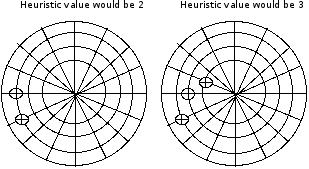
\includegraphics[width=4in]{heu.png}
\end{center}
\caption{Simple Heuristic Examples}
\label{heuristicExample}
\end{figure}

\subsection{Win Checking with Resolution}
The win checker used in the experiment determined a win, lose, or tie by using first order logic, resolution and unification.

\begin{table}
\begin{center}
\begin{tabular}{|c||c|}
\hline
player = p & north east neighbor = urn 
(for upper right neighbor)\\
\hline 
neighbor = n & north west neighbor = uln
(for upper left neighbor)\\
\hline 
left neighbor = ln & south east neighbor = drn
(for down right neighbor)\\
\hline 
right neighbor = rn & south west neighbor = dln
(for down left neighbor)\\
\hline 
upper neighbor = un & \\
\hline 
down neighbor = dn & \\
\hline 
\end{tabular}
\end{center}
\caption{Notation used in winchecker}
\label{Notation}
\end{table}


Let p = X \bigoplus O

Let connected = 4 be a winning state If n is moved on by p, perform a local search with that node as the origin.

\exists n \ni p \in {O,X} \bigwedge p \in n

An example of one of the sections of logic would be the check horizontal portion.

check left:
n \in \{a1, a2, a3, a4\} \Rightarrow ln \in \{l1, l2, l3, l4\}

\neg n \in \{a1, a2, a3, a4\} \bigwedge (n-1) \geqslant 0 \bigwedge p \in (n-1) \Rightarrow connected

check right:

n \in \{l1, l2, l3, l4\} \Rightarrow rn \in \{a1, a2, a3, a4\}

\neg n \in \{l1, l2, l3, l4\} \bigwedge (n+1) \leqslant 47 \bigwedge p \in (n+1) \Rightarrow connected

While for each of the logic checks a connected value of 4 is not found it goes through the other 3 first order rules. If at the end no winner has been found, connected = 0, It then becomes the other player’s turn.

\subsection{Game Evaluation with Classifiers}
Classifing the board is done with a Naive Bayes network. 

\subsection{Temproal Diffrence Neural Network}
When training the TDNN the first 20 games are trained against a random player. This is in hopes of reducing the risk of falling into an early local minimum. The remainder of n games chosen to be trained by a user is than done by pitting the current TDNN against itself. After each game is played the final result is evaluated and each state leading up to the result is compared to the prediction given by the network. Gradient descent is than done using the error of the network and allowing for adjustments to be made to the networks weights. The following equation is used to adjust weights in the network. 
\[
{\triangle} w_t = \alpha (V _{t + 1} - V _t)  \overset{t}{\sum_{k = 1}} {\gamme}^{t - k} {\nabla}_w V_k
\]
Where alpha is the learning rate and V is the perdicted output.

For each game the network is trained for both players, having the weights adjusted from both players perspectives after each game has ended.

The topology of the network is 48 inputs, one hidden layer with 40 nodes, and 3 output nodes. 48 input nodes to represent each possible state for a move and 3 output nodes; one for player 1 win, one for player 2 win, and one for a tie perdicted. 

\section{Experimental Methods}
In conducting experiments with the implemented algorithms we had them compete against each other 1000 games each. All algorithms competed against the other 3 and also against a random player. To get the performance result of using alpha beta pruning on minimax, it will also compete against the other 3 algorithms and against a random player while using alpha beta pruning. 


\newpage
\section{Results}

The results section should contain your results.  It should \emph{not} contain
your interpretation of those results.  That comes later.  This section should be
made up primarily of graphs and tables that show your data.  You should also
have a small amount of text describing what each of the tables and graphs shows,
since the caption on the figures should be short.  Having text describing the
specifics of the experiment that led to that particular table would also be
good.  

I am not going to tell you exactly what tables or graphs you should have here,
since it will depend a bit on your results.  You should be sure that your
results section contains sufficient data to support your conclusions about the
relative strengths and weaknesses of the different algorithms.  You should also
be sure that your data is complete; that is, do not leave data out simply because
it does not support the point you are trying to make.

You should also be sure that your results are clear and interpretable.  Seven
pages of raw binary data will do nothing to edify your reader.  Similarly, a
1 inch square graph with 12 lines plotted on it will be difficult to extract
meaning from, as will a graph with poor (or no) labels on the axes.  Your
results should be legible both on screen and in hard copy. By the way, do
not rely on color difference to make your points since many people read
black-and-white print outs of the papers (including your instructor).

You do not want to present results that are just raw data, since that is hard to
interpret.  But you do not want to be overly abstract, either, since that leads to
results that have little or no meaning (e.g., ``the average over all different
data sets, algorithms, and parameters'' is a completely useless statistic for
comparing algorithms).

\begin{table}
\begin{center}
\begin{tabular}{|c||c|c|c|c|}
\hline
& vs & win & tie & loss\\
\hline \hline
TDNN & Minimax & 0 & 0 & 1000\\
\hline 
TDNN & Simple Heuristic & 0 & 0 & 1000\\
\hline 
TDNN & Navie Bayes & 507 & 0 & 493\\
\hline 
TDNN & Random & 948 & 0 & 52\\
\hline 
\end{tabular}
\end{center}
\caption{Tempral Diffrence Neural Network performance with 40 hidden nodes}
\label{TDNNtable}
\end{table}

\begin{table}
\begin{center}
\begin{tabular}{|c||c|c|c|c|}
\hline
& vs & win & tie & loss\\
\hline \hline
Minimax & TDNN & 1000 & 0 & 0\\
\hline 
Minimax & Simple Heuristic & 476 & 0 & 524\\
\hline 
Minimax & Navie Bayes & 1000 & 0 & 0\\
\hline 
Minimax & Random & 979 & 1 & 20\\
\hline 
Minimax with Pruning & TDNN & 1000 & 0 & 0\\
\hline 
Minimax with Pruning & Simple Heuristic & 474 & 0 & 526\\
\hline 
Minimax with Pruning & Naive Bayes & 1000 & 0 & 0\\
\hline 
Minimax with Pruning & Random & 982 & 1 & 17\\
\hline 
\end{tabular}
\end{center}
\caption{Minimax Performance with depth of 2}
\label{MinimaxTable}
\end{table}


\begin{table}
\begin{center}
\begin{tabular}{|c||c|c|c|c|}
\hline
& vs & win & tie & loss\\
\hline \hline
Naive Bayes & TDNN & 487 & 0 & 513\\
\hline 
Naive Bayes & Simple Heuristic & 0 & 0 & 1000\\
\hline 
Naive Bayes & Minimax & 0 & 0 & 1000\\
\hline 
Naive Bayes & Random & 936 & 1 & 64\\
\hline 
\end{tabular}
\end{center}
\caption{Naive Bayes Performance}
\label{NaiveBayesTable}
\end{table}

\begin{table}
\begin{center}
\begin{tabular}{|c||c|c|c|c|}
\hline
& vs & win & tie & loss\\
\hline \hline
Simple Heuristic & TDNN & 1000 & 0 & 03\\
\hline 
Simple Heuristic & Minimax & 494 & 0 & 506\\
\hline 
Simple Heuristic & Naive Bayes & 1000 & 0 & 0\\
\hline 
Simple Heuristic & Random & 991 & 0 & 9\\
\hline 
\end{tabular}
\end{center}
\caption{Simple Heuristic Performance}
\label{HeuristicTable}
\end{table}

\begin{table}
\begin{center}
\begin{tabular}{|c||c|}
\hline
& win percentage\\
\hline \hline
TDNN & 36.4\\
\hline 
Simple Heuristic & 87.1\\
\hline 
Naive Bayes & 35.6\\
\hline 
Minimax & 86.4\\
\hline 
Minimax with Pruning & 86.4\\
\hline 
Random & 3.6\\
\hline 
\end{tabular}
\end{center}
\caption{Win percentage of algorithms in experiment}
\label{WinPercentTable}
\end{table}

\begin{figure}
\begin{center}
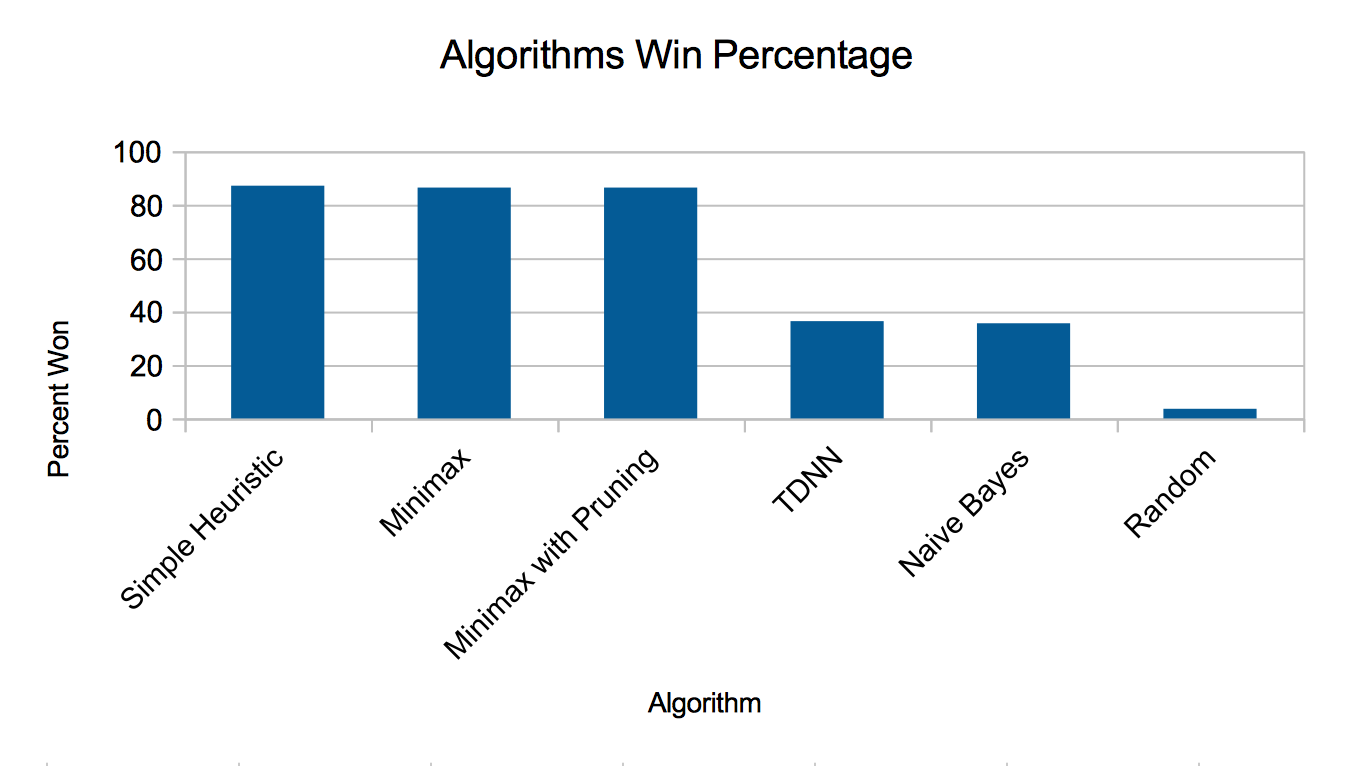
\includegraphics[width=7in]{winpercent.png}
\end{center}
\caption{Win Percentage}
\label{WinGraph}
\end{figure}

\section{Discussion}
In all of the tests the Simple Heuristic and the Minimax algorithms outperformed the TDNN and the Naive Bayes network. This pattern was consistent through out all of the tests that were ran. All algorithms were able to do better than random but that does not provide us with much information about the performance of the algorithm. 

\section{Conclusions}
While conducting the experiment it was shown that the simple heuristic and minimax algorthims performed best out of all of the implementations. It was also apparant while running the experiments that the Minimax tree gets very large relatively quickly when stored. The results lead to the suspicion that the topology of the TDNN is a large factor in it's ability to perform well.

In the experiment the TDNN did not perform well. We think this could be due to the amount of input nodes in comparision to the number of hidden nodes used. To test this we briefly ran a network that had 160 hidden nodes but still did not see a performance gain. Future exploration of the reason for it's lack of performance could be done in investigating the effect of having 48 input values. It may increase performance to do calculations to reduce the number of inputs since the state search space for backgammon in which it excelled was only 20. 



\newpage

\bibliographystyle{plain}
\bibliography{reffrences}
\nocite{*}

\end{document}
